\subsubsection{Auxiliary Operations}

In this subsection, we describe useful auxiliary operations.

\subsubsubsection{cubMap}

The method \operator{cubMap} implements the cubic map of a set. Given a set $\mathcal{S} \subset \Rn$, the cubic map is defined as 
\begin{equation*}
	\operator{cubMap}(\mathcal{S},Q) = \bigg \{ x ~ \bigg | ~ x_{(i)} = \sum_{j=1}^n s_{(j)} ~(s^T ~T_{i,j}~ s), ~s \in \mathcal{S},~ i = 1 \dots w \bigg \}, ~ T_{i,j} \in \R^{n \times n},
\end{equation*}
where $x_{(i)}$ is the $i$-th value of the vector $x$. If the corresponding set representation is not closed under cubic maps, \operator{cubMap} returns an over-approximation. If \operator{cubMap} is called with three different sets $\mathcal{S}_1,\mathcal{S}_2,\mathcal{S}_3 \subset \Rn$ as input arguments, the method computes the mixed cubic map:
\begin{equation*}
\begin{split}
	\operator{cubMap}(\mathcal{S}_1,\mathcal{S}_2,\mathcal{S}_3,Q) = \bigg \{ x ~ \bigg | ~ & x_{(i)} = \sum_{j=1}^n s_{1(j)} ~(s_2^T ~T_{i,j}~ s_3), ~s_1 \in \mathcal{S}_1,~s_2 \in \mathcal{S}_2,~s_3 \in \mathcal{S}_3, \\
	& i = 1 \dots w \bigg \}, ~ T_{i,j} \in \R^{n \times n},
\end{split}
\end{equation*}
Let us demonstrate the method $\operator{cubMap}$ by an example:

\begin{center}
\begin{minipage}[t]{0.35\textwidth}
	\vspace{10pt}
	\footnotesize
	\definecolor{mycolor1}{rgb}{0.00000,0.44700,0.74100}%
\definecolor{mycolor2}{rgb}{0.46600,0.67400,0.18800}%
%
\begin{tikzpicture}
\footnotesize
\pgfplotsset{
plotstyle1/.style={color=mycolor1, forget plot},
plotstyle2/.style={color=mycolor2, forget plot}
}
\def\rows{1}
\def\cols{2}
\def\horzsep{1cm}
\def\basepath{./figures/tikz/set-operations-aux/}

\begin{groupplot}[%
group style={rows = \rows, columns = \cols, horizontal sep = \horzsep},
scale only axis,
width=1/\cols*\textwidth -\horzsep,
legend style={legend columns=2,legend to name=legendname, legend cell align=left,/tikz/every even column/.append style={column sep=0.5cm}}
]
\nextgroupplot[xmin=-3,xmax=3,ymin=-3,ymax=3,xlabel={$x_{(1)}$},ylabel={$x_{(2)}$},title={$\mathcal{S}$}]
\input{\basepath example_cubMap_11.tikz}
\coordinate (top) at (rel axis cs:0,1);
\nextgroupplot[xmin=-3,xmax=3,ymin=-3,ymax=3,xlabel={$x_{(1)}$},title={$\texttt{cubMap}(\mathcal{S},T)$}]
\input{\basepath example_cubMap_legends.tikz}
\input{\basepath example_cubMap_12.tikz}
\coordinate (bot) at (rel axis cs:1,0);
\end{groupplot}
\path (top|-current bounding box.south)--coordinate(legendpos)(bot|-current bounding box.south);
\node at([yshift=-6ex]legendpos) {\pgfplotslegendfromname{legendname}};

\end{tikzpicture}%
\end{minipage}
\begin{minipage}[t]{0.6\textwidth}
	\vspace{0pt}
	\centering
	\includetikz{./figures/tikz/set-operations-aux/example_cubMap}
\end{minipage}
\end{center}


\subsubsubsection{enclose}

The method \operator{enclose} computes an enclosure of a set and its linear transformation. Given the sets $\mathcal{S}_1,\mathcal{S}_2 \in \Rn$ and the matrix $M \in \R^{n \times n}$, \operator{enclose} computes the set
\begin{equation}
	\operator{enclose}(\mathcal{S}_1,M,\mathcal{S}_2) = \left \{ \lambda s_1 + (1-\lambda) (Ms_1 +s_2) ~|~ s_1 \in \mathcal{S}_1,~s_2 \in \mathcal{S}_2,~\lambda \in [0,1] \right\}.
	\label{eq:enclose}
\end{equation}
If the set as defined in \eqref{eq:enclose} cannot be computed exactly for the corresponding set representation, \operator{enclose} returns an over-approximation. For convenience, the method can also be called with only two input arguments:
\begin{equation*}
	\operator{enclose}(\mathcal{S}_1,\mathcal{S}_3) = \operator{enclose}(\mathcal{S}_1,M,\mathcal{S}_2), ~~~ \mathcal{S}_3 = (M \otimes \mathcal{S}_1) \oplus \mathcal{S}_2.
\end{equation*}
Let us demonstrate the method $\operator{enclose}$ by an example:

\begin{center}
\begin{minipage}[t]{0.37\textwidth}
	\vspace{10pt}
	\footnotesize
	% This file was automatically created from the m-file 
% "m2tex.m" written by USL. 
% The fontencoding in this file is UTF-8. 
%  
% You will need to include the following two packages in 
% your LaTeX-Main-File. 
%  
% \usepackage{color} 
% \usepackage{fancyvrb} 
%  
% It is advised to use the following option for Inputenc 
% \usepackage[utf8]{inputenc} 
%  
  
% definition of matlab colors: 
\definecolor{mblue}{rgb}{0,0,1} 
\definecolor{mgreen}{rgb}{0.13333,0.5451,0.13333} 
\definecolor{mred}{rgb}{0.62745,0.12549,0.94118} 
\definecolor{mgrey}{rgb}{0.5,0.5,0.5} 
\definecolor{mdarkgrey}{rgb}{0.25,0.25,0.25} 
  
\DefineShortVerb[fontfamily=courier,fontseries=m]{\$} 
\DefineShortVerb[fontfamily=courier,fontseries=b]{\#} 
  
\noindent            
 $$\color{mgreen}$% sets S1,S2 and matrix M$\color{black}$$\\
 $S1 = polyZonotope([1.5;1.5],$\color{mblue}$ ...$\color{black}$$\\
 $                  [1 0;0 1],$\color{mblue}$ ...$\color{black}$$\\
 $                  [],eye(2));$\\
 $S2 = [0.5;0.5];$\\
 $M = [-1 0;0 -1];$\\
 $           $\\
 $$\color{mgreen}$% apply method enclose$\color{black}$$\\
 $S3 = M*S1 + S2;$\\
 $$\\
 $res = enclose(S1,M,S2);$\\
 $res = enclose(S1,S3);$\\ 
  
\UndefineShortVerb{\$} 
\UndefineShortVerb{\#}
\end{minipage}
\begin{minipage}[t]{0.6\textwidth}
	\vspace{0pt}
	\centering
	\includetikz{./figures/tikz/set-operations-aux/example_enclose}
\end{minipage}
\end{center}

\vspace{1cm}

\subsubsubsection{enclosePoints}

Given a point cloud $P = [p_1,\dots,p_m]$, $p_i \in \Rn$, the static method \operator{enclosePoints} computes a set $\mathcal{S} \subset \Rn$ that tightly encloses the point cloud:
\begin{equation*}
	\mathcal{S} = \operator{enclosePoints}\big([p_1,\dots,p_m]\big), ~~ \forall i = 1,\dots,m: ~ p_i \in \mathcal{S}.
\end{equation*}

Let us demonstrate the method \operator{enclosePoints} by an example:

\begin{center}
\begin{minipage}[t]{0.50\textwidth}
	\vspace{10pt}
	\footnotesize
	% This file was created by matlab2tikz.
%
\definecolor{mycolor1}{rgb}{0.00000,0.44700,0.74100}%
%
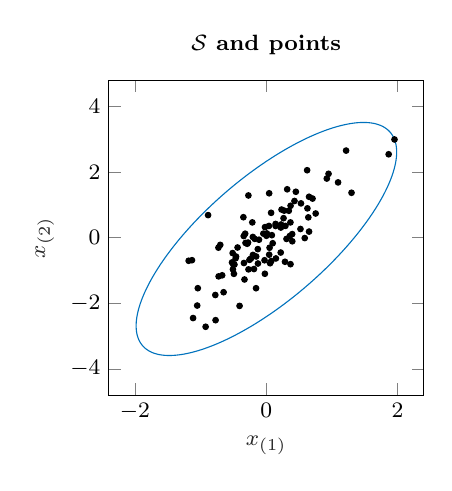
\begin{tikzpicture}
\footnotesize

\begin{axis}[%
width=4cm,
height=4cm,
at={(0in,0in)},
scale only axis,
xmin=-2.4,
xmax=2.4,
xlabel style={font=\color{white!15!black}},
xlabel={$x_{(1)}$},
ymin=-4.8,
ymax=4.8,
ylabel style={font=\color{white!15!black}},
ylabel={$x_{(2)}$},
axis background/.style={fill=white},
title style={font=\bfseries},
title={$\mathcal{S}$ and points}
]
\addplot [color=mycolor1, forget plot]
  table[row sep=crcr]{%
-1.6544	-3.5538\\
-1.6565	-3.5527\\
-1.6586	-3.5517\\
-1.6607	-3.5506\\
-1.6629	-3.5496\\
-1.6734	-3.5441\\
-1.6754	-3.5429\\
-1.6775	-3.5417\\
-1.6796	-3.5406\\
-1.6817	-3.5394\\
-1.6837	-3.5382\\
-1.6858	-3.537\\
-1.6879	-3.5357\\
-1.6899	-3.5345\\
-1.692	-3.5332\\
-1.696	-3.5306\\
-1.6981	-3.5293\\
-1.7001	-3.528\\
-1.7021	-3.5266\\
-1.7042	-3.5253\\
-1.7122	-3.5197\\
-1.7143	-3.5182\\
-1.7163	-3.5168\\
-1.7223	-3.5123\\
-1.7243	-3.5107\\
-1.7263	-3.5092\\
-1.7303	-3.506\\
-1.7322	-3.5044\\
-1.7362	-3.5012\\
-1.7442	-3.4944\\
-1.7461	-3.4926\\
-1.7481	-3.4909\\
-1.7521	-3.4873\\
-1.754	-3.4854\\
-1.756	-3.4836\\
-1.76	-3.4798\\
-1.7659	-3.4739\\
-1.7678	-3.4719\\
-1.7718	-3.4679\\
-1.7738	-3.4658\\
-1.7757	-3.4637\\
-1.7777	-3.4616\\
-1.7797	-3.4594\\
-1.7816	-3.4572\\
-1.7856	-3.4528\\
-1.7875	-3.4505\\
-1.7915	-3.4459\\
-1.7935	-3.4435\\
-1.7954	-3.4412\\
-1.7974	-3.4387\\
-1.7994	-3.4363\\
-1.8013	-3.4338\\
-1.8033	-3.4313\\
-1.8053	-3.4287\\
-1.8073	-3.4262\\
-1.8092	-3.4235\\
-1.8112	-3.4209\\
-1.8152	-3.4155\\
-1.8171	-3.4127\\
-1.8211	-3.4071\\
-1.8251	-3.4013\\
-1.8271	-3.3983\\
-1.829	-3.3953\\
-1.831	-3.3923\\
-1.833	-3.3892\\
-1.839	-3.3796\\
-1.843	-3.373\\
-1.845	-3.3696\\
-1.8469	-3.3662\\
-1.8509	-3.3592\\
-1.8549	-3.352\\
-1.8589	-3.3446\\
-1.8609	-3.3408\\
-1.8649	-3.333\\
-1.8669	-3.329\\
-1.8709	-3.3208\\
-1.8749	-3.3124\\
-1.8809	-3.2992\\
-1.8849	-3.29\\
-1.8889	-3.2806\\
-1.8909	-3.2757\\
-1.8928	-3.2708\\
-1.8968	-3.2606\\
-1.8988	-3.2554\\
-1.9008	-3.2501\\
-1.9027	-3.2447\\
-1.9047	-3.2393\\
-1.9067	-3.2337\\
-1.9086	-3.228\\
-1.9106	-3.2222\\
-1.9125	-3.2163\\
-1.9145	-3.2103\\
-1.9164	-3.2042\\
-1.9184	-3.198\\
-1.9222	-3.1852\\
-1.9241	-3.1786\\
-1.9279	-3.165\\
-1.9298	-3.158\\
-1.9317	-3.1509\\
-1.9335	-3.1436\\
-1.9354	-3.1362\\
-1.9372	-3.1287\\
-1.939	-3.121\\
-1.9408	-3.1131\\
-1.9426	-3.1051\\
-1.9444	-3.0969\\
-1.9461	-3.0886\\
-1.9479	-3.08\\
-1.9496	-3.0713\\
-1.9513	-3.0624\\
-1.9529	-3.0534\\
-1.9546	-3.0441\\
-1.9562	-3.0346\\
-1.9578	-3.0249\\
-1.9593	-3.015\\
-1.9609	-3.0049\\
-1.9624	-2.9946\\
-1.9638	-2.984\\
-1.9653	-2.9732\\
-1.9666	-2.9622\\
-1.968	-2.9509\\
-1.9693	-2.9393\\
-1.9706	-2.9275\\
-1.9718	-2.9154\\
-1.9729	-2.903\\
-1.974	-2.8904\\
-1.9751	-2.8774\\
-1.9761	-2.8641\\
-1.977	-2.8505\\
-1.9779	-2.8366\\
-1.9787	-2.8224\\
-1.9794	-2.8078\\
-1.9801	-2.7928\\
-1.9806	-2.7775\\
-1.9811	-2.7618\\
-1.9815	-2.7457\\
-1.9818	-2.7292\\
-1.982	-2.7123\\
-1.9821	-2.6949\\
-1.9821	-2.6771\\
-1.982	-2.6589\\
-1.9817	-2.6402\\
-1.9813	-2.621\\
-1.9808	-2.6013\\
-1.9802	-2.5811\\
-1.9794	-2.5604\\
-1.9784	-2.5391\\
-1.9773	-2.5173\\
-1.976	-2.4949\\
-1.9746	-2.4719\\
-1.9729	-2.4483\\
-1.9711	-2.4241\\
-1.969	-2.3992\\
-1.9668	-2.3736\\
-1.9643	-2.3474\\
-1.9615	-2.3205\\
-1.9585	-2.2928\\
-1.9553	-2.2644\\
-1.9518	-2.2353\\
-1.948	-2.2053\\
-1.9439	-2.1746\\
-1.9395	-2.143\\
-1.9347	-2.1106\\
-1.9296	-2.0773\\
-1.9242	-2.0431\\
-1.9184	-2.008\\
-1.9122	-1.972\\
-1.9056	-1.935\\
-1.8986	-1.8971\\
-1.8912	-1.8582\\
-1.8832	-1.8183\\
-1.8749	-1.7773\\
-1.866	-1.7353\\
-1.8566	-1.6923\\
-1.8468	-1.6482\\
-1.8363	-1.603\\
-1.8253	-1.5567\\
-1.8137	-1.5093\\
-1.8016	-1.4607\\
-1.7888	-1.4111\\
-1.7754	-1.3603\\
-1.7613	-1.3083\\
-1.7466	-1.2553\\
-1.7312	-1.2011\\
-1.7151	-1.1458\\
-1.6982	-1.0894\\
-1.6807	-1.0318\\
-1.6624	-0.9732\\
-1.6434	-0.9135\\
-1.6236	-0.8528\\
-1.6031	-0.791\\
-1.5818	-0.7283\\
-1.5597	-0.6646\\
-1.5368	-0.6\\
-1.5132	-0.5345\\
-1.4888	-0.4682\\
-1.4637	-0.4012\\
-1.4378	-0.3334\\
-1.4111	-0.265\\
-1.3838	-0.1959\\
-1.3557	-0.1264\\
-1.3269	-0.0564\\
-1.2974	0.014\\
-1.2673	0.0847\\
-1.2365	0.1557\\
-1.2052	0.2267\\
-1.1732	0.2979\\
-1.1408	0.3691\\
-1.1078	0.4401\\
-1.0744	0.5111\\
-1.0406	0.5817\\
-1.0063	0.652\\
-0.9718	0.7219\\
-0.9369	0.7914\\
-0.9017	0.8602\\
-0.8664	0.9285\\
-0.8308	0.996\\
-0.7951	1.0628\\
-0.7594	1.1287\\
-0.7236	1.1938\\
-0.6877	1.2579\\
-0.652	1.321\\
-0.6162	1.3831\\
-0.5806	1.4441\\
-0.5451	1.5039\\
-0.5099	1.5627\\
-0.4748	1.6202\\
-0.44	1.6766\\
-0.4054	1.7318\\
-0.3711	1.7857\\
-0.3372	1.8383\\
-0.3036	1.8897\\
-0.2704	1.9399\\
-0.2376	1.9888\\
-0.2052	2.0364\\
-0.1732	2.0828\\
-0.1416	2.1279\\
-0.1105	2.1718\\
-0.0799	2.2145\\
-0.0497	2.2559\\
-0.02	2.2962\\
0.0092	2.3353\\
0.0379	2.3733\\
0.0661	2.4101\\
0.0938	2.4458\\
0.1211	2.4804\\
0.1478	2.514\\
0.1741	2.5465\\
0.1998	2.578\\
0.2251	2.6085\\
0.2499	2.6381\\
0.2742	2.6667\\
0.2981	2.6944\\
0.3214	2.7212\\
0.3443	2.7471\\
0.3668	2.7722\\
0.3888	2.7965\\
0.4103	2.82\\
0.4314	2.8427\\
0.4521	2.8647\\
0.4723	2.886\\
0.4922	2.9066\\
0.5116	2.9265\\
0.5307	2.9457\\
0.5493	2.9643\\
0.5676	2.9824\\
0.5854	2.9998\\
0.603	3.0166\\
0.6201	3.0329\\
0.6369	3.0487\\
0.6534	3.0639\\
0.6695	3.0787\\
0.6853	3.0929\\
0.7008	3.1067\\
0.716	3.1201\\
0.7308	3.133\\
0.7454	3.1455\\
0.7596	3.1576\\
0.7736	3.1693\\
0.7873	3.1807\\
0.8008	3.1916\\
0.814	3.2022\\
0.8269	3.2125\\
0.8396	3.2224\\
0.852	3.2321\\
0.8642	3.2414\\
0.8761	3.2504\\
0.8878	3.2591\\
0.8993	3.2676\\
0.9106	3.2758\\
0.9217	3.2837\\
0.9326	3.2914\\
0.9432	3.2988\\
0.9537	3.306\\
0.964	3.313\\
0.9741	3.3198\\
0.984	3.3263\\
0.9938	3.3327\\
1.0033	3.3388\\
1.0127	3.3448\\
1.022	3.3506\\
1.0311	3.3562\\
1.04	3.3616\\
1.0488	3.3668\\
1.0574	3.3719\\
1.0659	3.3769\\
1.0742	3.3816\\
1.0824	3.3863\\
1.0905	3.3908\\
1.0984	3.3951\\
1.1062	3.3994\\
1.1139	3.4034\\
1.1214	3.4074\\
1.1289	3.4113\\
1.1362	3.415\\
1.1434	3.4186\\
1.1505	3.4221\\
1.1575	3.4255\\
1.1644	3.4288\\
1.1712	3.432\\
1.1844	3.438\\
1.1909	3.4409\\
1.1973	3.4437\\
1.2036	3.4465\\
1.2098	3.4491\\
1.222	3.4541\\
1.2279	3.4565\\
1.2338	3.4588\\
1.2396	3.4611\\
1.2453	3.4633\\
1.2509	3.4654\\
1.2565	3.4674\\
1.262	3.4694\\
1.2674	3.4713\\
1.278	3.4749\\
1.2832	3.4766\\
1.2883	3.4783\\
1.2934	3.4799\\
1.2984	3.4815\\
1.3034	3.483\\
1.3082	3.4844\\
1.3131	3.4858\\
1.3179	3.4872\\
1.3226	3.4885\\
1.3364	3.4921\\
1.3409	3.4932\\
1.3453	3.4943\\
1.3541	3.4963\\
1.3584	3.4973\\
1.3668	3.4991\\
1.371	3.4999\\
1.3792	3.5015\\
1.3832	3.5023\\
1.3872	3.503\\
1.3912	3.5036\\
1.3951	3.5043\\
1.3989	3.5049\\
1.4028	3.5055\\
1.4066	3.506\\
1.4177	3.5075\\
1.4214	3.5079\\
1.4286	3.5087\\
1.4321	3.5091\\
1.4426	3.51\\
1.446	3.5103\\
1.4494	3.5105\\
1.4527	3.5107\\
1.4561	3.5109\\
1.4594	3.511\\
1.4627	3.5112\\
1.4723	3.5115\\
1.4755	3.5115\\
1.4786	3.5116\\
1.4879	3.5116\\
1.491	3.5115\\
1.494	3.5115\\
1.5	3.5113\\
1.5029	3.5112\\
1.5059	3.5111\\
1.5117	3.5107\\
1.5145	3.5106\\
1.5174	3.5104\\
1.5202	3.5101\\
1.5258	3.5097\\
1.5314	3.5091\\
1.5395	3.5082\\
1.5422	3.5078\\
1.5449	3.5075\\
1.5476	3.5071\\
1.558	3.5055\\
1.5606	3.505\\
1.5632	3.5046\\
1.5682	3.5036\\
1.5708	3.5031\\
1.5758	3.5021\\
1.5782	3.5016\\
1.5832	3.5004\\
1.5856	3.4999\\
1.588	3.4993\\
1.5905	3.4987\\
1.5929	3.498\\
1.5953	3.4974\\
1.5976	3.4968\\
1.6024	3.4954\\
1.6047	3.4947\\
1.6071	3.494\\
1.614	3.4919\\
1.6163	3.4911\\
1.6186	3.4904\\
1.6232	3.4888\\
1.6254	3.488\\
1.6277	3.4872\\
1.6299	3.4864\\
1.6322	3.4855\\
1.6344	3.4847\\
1.6498	3.4784\\
1.6519	3.4774\\
1.6541	3.4764\\
1.6562	3.4754\\
1.6584	3.4744\\
1.6605	3.4734\\
1.6627	3.4724\\
1.6648	3.4714\\
1.6669	3.4703\\
1.669	3.4693\\
1.6774	3.4649\\
1.6795	3.4637\\
1.6816	3.4626\\
1.6837	3.4614\\
1.6858	3.4603\\
1.6878	3.4591\\
1.6899	3.4579\\
1.692	3.4566\\
1.694	3.4554\\
1.6961	3.4542\\
1.6981	3.4529\\
1.7002	3.4516\\
1.7042	3.449\\
1.7063	3.4477\\
1.7083	3.4463\\
1.7103	3.445\\
1.7124	3.4436\\
1.7184	3.4394\\
1.7224	3.4364\\
1.7244	3.435\\
1.7284	3.432\\
1.7304	3.4304\\
1.7324	3.4289\\
1.7404	3.4225\\
1.7424	3.4208\\
1.7444	3.4192\\
1.7464	3.4175\\
1.7483	3.4158\\
1.7503	3.4141\\
1.7563	3.4087\\
1.7582	3.4069\\
1.7602	3.4051\\
1.7622	3.4032\\
1.7642	3.4014\\
1.7681	3.3975\\
1.7701	3.3956\\
1.772	3.3936\\
1.776	3.3896\\
1.778	3.3875\\
1.7799	3.3855\\
1.7819	3.3834\\
1.7839	3.3812\\
1.7858	3.3791\\
1.7898	3.3747\\
1.7917	3.3725\\
1.7957	3.3679\\
1.7976	3.3656\\
1.8036	3.3584\\
1.8055	3.356\\
1.8095	3.351\\
1.8115	3.3484\\
1.8134	3.3458\\
1.8174	3.3406\\
1.8194	3.3379\\
1.8213	3.3352\\
1.8273	3.3268\\
1.8293	3.3239\\
1.8312	3.321\\
1.8352	3.315\\
1.8412	3.3057\\
1.8432	3.3025\\
1.8451	3.2993\\
1.8491	3.2927\\
1.8531	3.2859\\
1.8571	3.2789\\
1.8611	3.2717\\
1.8631	3.268\\
1.8691	3.2566\\
1.8711	3.2526\\
1.8731	3.2487\\
1.8771	3.2405\\
1.8791	3.2363\\
1.8831	3.2277\\
1.8871	3.2189\\
1.8891	3.2143\\
1.891	3.2097\\
1.893	3.205\\
1.897	3.1954\\
1.901	3.1854\\
1.903	3.1803\\
1.905	3.1751\\
1.9069	3.1698\\
1.9089	3.1644\\
1.9109	3.1589\\
1.9128	3.1534\\
1.9148	3.1477\\
1.9168	3.1419\\
1.9187	3.136\\
1.9207	3.13\\
1.9226	3.1239\\
1.9245	3.1176\\
1.9265	3.1113\\
1.9284	3.1048\\
1.9303	3.0982\\
1.9322	3.0915\\
1.9341	3.0847\\
1.936	3.0777\\
1.9378	3.0706\\
1.9397	3.0633\\
1.9415	3.0559\\
1.9434	3.0484\\
1.9452	3.0407\\
1.947	3.0328\\
1.9488	3.0248\\
1.9505	3.0166\\
1.9523	3.0083\\
1.954	2.9997\\
1.9557	2.991\\
1.9574	2.9821\\
1.9591	2.9731\\
1.9607	2.9638\\
1.9624	2.9543\\
1.9639	2.9446\\
1.9655	2.9347\\
1.967	2.9246\\
1.9685	2.9143\\
1.97	2.9037\\
1.9714	2.8929\\
1.9728	2.8819\\
1.9742	2.8706\\
1.9755	2.859\\
1.9767	2.8472\\
1.9779	2.8351\\
1.9791	2.8227\\
1.9802	2.8101\\
1.9813	2.7971\\
1.9823	2.7838\\
1.9832	2.7702\\
1.9841	2.7563\\
1.9848	2.7421\\
1.9856	2.7275\\
1.9862	2.7125\\
1.9868	2.6972\\
1.9873	2.6815\\
1.9877	2.6654\\
1.988	2.6489\\
1.9882	2.6319\\
1.9883	2.6146\\
1.9883	2.5968\\
1.9881	2.5786\\
1.9879	2.5599\\
1.9875	2.5407\\
1.987	2.521\\
1.9864	2.5008\\
1.9856	2.4801\\
1.9846	2.4588\\
1.9835	2.437\\
1.9822	2.4146\\
1.9807	2.3916\\
1.9791	2.368\\
1.9773	2.3437\\
1.9752	2.3189\\
1.9729	2.2933\\
1.9704	2.2671\\
1.9677	2.2402\\
1.9647	2.2125\\
1.9615	2.1841\\
1.958	2.1549\\
1.9541	2.125\\
1.95	2.0942\\
1.9456	2.0627\\
1.9409	2.0302\\
1.9358	1.997\\
1.9304	1.9628\\
1.9246	1.9277\\
1.9184	1.8917\\
1.9118	1.8547\\
1.9048	1.8168\\
1.8973	1.7779\\
1.8894	1.738\\
1.881	1.697\\
1.8722	1.655\\
1.8628	1.612\\
1.8529	1.5679\\
1.8425	1.5227\\
1.8315	1.4764\\
1.8199	1.4289\\
1.8077	1.3804\\
1.795	1.3307\\
1.7815	1.2799\\
1.7675	1.228\\
1.7527	1.175\\
1.7373	1.1208\\
1.7212	1.0655\\
1.7044	1.009\\
1.6869	0.9515\\
1.6686	0.8929\\
1.6496	0.8332\\
1.6298	0.7725\\
1.6092	0.7107\\
1.5879	0.648\\
1.5659	0.5843\\
1.543	0.5197\\
1.5194	0.4542\\
1.495	0.3879\\
1.4699	0.3209\\
1.444	0.2531\\
1.4173	0.1847\\
1.3899	0.1156\\
1.3618	0.0461\\
1.333	-0.0239\\
1.3036	-0.0943\\
1.2734	-0.165\\
1.2427	-0.236\\
1.2113	-0.3071\\
1.1794	-0.3782\\
1.147	-0.4494\\
1.114	-0.5205\\
1.0806	-0.5914\\
1.0467	-0.662\\
1.0125	-0.7323\\
0.9779	-0.8023\\
0.943	-0.8717\\
0.9079	-0.9405\\
0.8725	-1.0088\\
0.837	-1.0763\\
0.8013	-1.1431\\
0.7655	-1.209\\
0.7297	-1.2741\\
0.6939	-1.3382\\
0.6581	-1.4013\\
0.6224	-1.4634\\
0.5868	-1.5244\\
0.5513	-1.5843\\
0.516	-1.643\\
0.481	-1.7006\\
0.4461	-1.7569\\
0.4116	-1.8121\\
0.3773	-1.866\\
0.3434	-1.9186\\
0.3098	-1.97\\
0.2766	-2.0202\\
0.2438	-2.0691\\
0.2113	-2.1167\\
0.1794	-2.1631\\
0.1478	-2.2082\\
0.1167	-2.2521\\
0.0861	-2.2948\\
0.0559	-2.3362\\
0.0262	-2.3765\\
-0.003	-2.4156\\
-0.0317	-2.4536\\
-0.0599	-2.4904\\
-0.0877	-2.5261\\
-0.1149	-2.5607\\
-0.1417	-2.5943\\
-0.1679	-2.6268\\
-0.1937	-2.6583\\
-0.219	-2.6888\\
-0.2437	-2.7184\\
-0.2681	-2.747\\
-0.2919	-2.7747\\
-0.3153	-2.8015\\
-0.3382	-2.8274\\
-0.3606	-2.8525\\
-0.3826	-2.8768\\
-0.4041	-2.9003\\
-0.4252	-2.923\\
-0.4459	-2.945\\
-0.4662	-2.9663\\
-0.486	-2.9869\\
-0.5055	-3.0068\\
-0.5245	-3.026\\
-0.5431	-3.0447\\
-0.5614	-3.0627\\
-0.5793	-3.0801\\
-0.5968	-3.0969\\
-0.6139	-3.1132\\
-0.6308	-3.129\\
-0.6472	-3.1442\\
-0.6633	-3.159\\
-0.6791	-3.1733\\
-0.6946	-3.1871\\
-0.7098	-3.2004\\
-0.7246	-3.2133\\
-0.7392	-3.2258\\
-0.7535	-3.2379\\
-0.7675	-3.2496\\
-0.7812	-3.261\\
-0.7946	-3.2719\\
-0.8078	-3.2825\\
-0.8207	-3.2928\\
-0.8334	-3.3028\\
-0.8458	-3.3124\\
-0.858	-3.3217\\
-0.8699	-3.3307\\
-0.8817	-3.3394\\
-0.8932	-3.3479\\
-0.9045	-3.3561\\
-0.9155	-3.364\\
-0.9264	-3.3717\\
-0.9371	-3.3791\\
-0.9476	-3.3864\\
-0.9578	-3.3933\\
-0.9679	-3.4001\\
-0.9779	-3.4066\\
-0.9876	-3.413\\
-0.9972	-3.4191\\
-1.0066	-3.4251\\
-1.0158	-3.4309\\
-1.0249	-3.4365\\
-1.0338	-3.4419\\
-1.0426	-3.4472\\
-1.0512	-3.4522\\
-1.0597	-3.4572\\
-1.068	-3.462\\
-1.0762	-3.4666\\
-1.0843	-3.4711\\
-1.0922	-3.4754\\
-1.1	-3.4797\\
-1.1077	-3.4838\\
-1.1153	-3.4877\\
-1.1227	-3.4916\\
-1.13	-3.4953\\
-1.1372	-3.4989\\
-1.1443	-3.5024\\
-1.1513	-3.5058\\
-1.1582	-3.5091\\
-1.165	-3.5123\\
-1.1717	-3.5154\\
-1.1783	-3.5183\\
-1.1911	-3.5241\\
-1.1974	-3.5268\\
-1.2098	-3.532\\
-1.2158	-3.5344\\
-1.2276	-3.5392\\
-1.2334	-3.5414\\
-1.2391	-3.5436\\
-1.2447	-3.5457\\
-1.2503	-3.5477\\
-1.2558	-3.5497\\
-1.2612	-3.5516\\
-1.2718	-3.5552\\
-1.2822	-3.5586\\
-1.2922	-3.5618\\
-1.2972	-3.5633\\
-1.3021	-3.5647\\
-1.3117	-3.5675\\
-1.3164	-3.5688\\
-1.3211	-3.57\\
-1.3257	-3.5712\\
-1.3302	-3.5724\\
-1.3392	-3.5746\\
-1.3436	-3.5756\\
-1.3522	-3.5776\\
-1.3565	-3.5785\\
-1.3607	-3.5794\\
-1.3648	-3.5803\\
-1.369	-3.5811\\
-1.373	-3.5818\\
-1.3771	-3.5826\\
-1.3811	-3.5833\\
-1.385	-3.584\\
-1.3928	-3.5852\\
-1.3966	-3.5858\\
-1.4004	-3.5863\\
-1.4042	-3.5869\\
-1.4079	-3.5873\\
-1.4116	-3.5878\\
-1.4152	-3.5882\\
-1.4188	-3.5887\\
-1.4224	-3.589\\
-1.426	-3.5894\\
-1.433	-3.59\\
-1.4398	-3.5906\\
-1.4466	-3.591\\
-1.4532	-3.5914\\
-1.4565	-3.5915\\
-1.4597	-3.5916\\
-1.463	-3.5917\\
-1.4662	-3.5918\\
-1.4693	-3.5919\\
-1.4818	-3.5919\\
-1.4848	-3.5918\\
-1.4878	-3.5918\\
-1.4968	-3.5915\\
-1.4997	-3.5914\\
-1.5026	-3.5912\\
-1.5055	-3.5911\\
-1.5084	-3.5909\\
-1.5112	-3.5907\\
-1.5141	-3.5905\\
-1.5169	-3.5902\\
-1.5197	-3.59\\
-1.5225	-3.5897\\
-1.5279	-3.5891\\
-1.5307	-3.5888\\
-1.5361	-3.5882\\
-1.5387	-3.5878\\
-1.5414	-3.5874\\
-1.544	-3.587\\
-1.5467	-3.5866\\
-1.5519	-3.5858\\
-1.5544	-3.5854\\
-1.557	-3.5849\\
-1.5595	-3.5844\\
-1.5621	-3.5839\\
-1.5721	-3.5819\\
-1.5745	-3.5813\\
-1.577	-3.5807\\
-1.5794	-3.5802\\
-1.5819	-3.5796\\
-1.5867	-3.5784\\
-1.5891	-3.5777\\
-1.5915	-3.5771\\
-1.5938	-3.5764\\
-1.5962	-3.5757\\
-1.5985	-3.5751\\
-1.6009	-3.5744\\
-1.6032	-3.5737\\
-1.6055	-3.5729\\
-1.6078	-3.5722\\
-1.6101	-3.5714\\
-1.6124	-3.5707\\
-1.617	-3.5691\\
-1.6192	-3.5683\\
-1.6215	-3.5675\\
-1.6237	-3.5667\\
-1.626	-3.5658\\
-1.6282	-3.565\\
-1.6326	-3.5632\\
-1.6348	-3.5624\\
-1.637	-3.5615\\
-1.6392	-3.5605\\
-1.6436	-3.5587\\
-1.6458	-3.5577\\
-1.6479	-3.5567\\
-1.6501	-3.5558\\
-1.6522	-3.5548\\
-1.6544	-3.5538\\
};
\addplot[only marks, mark=*, mark options={}, mark size=1.0000pt, draw=black, forget plot] table[row sep=crcr]{%
x	y\\
-1.1816	-0.7045\\
-1.131	-0.6869\\
-1.1141	-2.4505\\
-1.0513	-2.0697\\
-1.042	-1.5404\\
-0.9228	-2.7159\\
-0.8854	0.6869\\
-0.7751	-1.7478\\
-0.7713	-2.5151\\
-0.7277	-0.3042\\
-0.7251	-1.1804\\
-0.7001	-0.2204\\
-0.671	-1.1476\\
-0.6491	-1.6635\\
-0.521	-0.7544\\
-0.5114	-0.4702\\
-0.5071	-0.9678\\
-0.5032	-0.8109\\
-0.4918	-1.1026\\
-0.4838	-0.8186\\
-0.4655	-0.63\\
-0.4591	-0.5763\\
-0.4362	-0.3001\\
-0.4057	-2.08\\
-0.3475	0.6234\\
-0.3422	0.0494\\
-0.3393	-0.7726\\
-0.3308	-1.2746\\
-0.3202	0.1211\\
-0.3149	-0.1607\\
-0.2892	-0.1862\\
-0.2766	-0.1494\\
-0.2711	1.2866\\
-0.2696	-0.9667\\
-0.2551	-0.6767\\
-0.2333	-0.6382\\
-0.2116	0.4655\\
-0.2036	0.0212\\
-0.202	-0.5263\\
-0.1864	-0.9563\\
-0.1752	-0.0357\\
-0.1547	-1.5411\\
-0.1527	-0.5738\\
-0.1278	-0.3494\\
-0.1256	-0.7882\\
-0.1098	-0.0629\\
-0.0434	0.123\\
-0.0252	-0.6889\\
-0.02	-1.1011\\
-0.0183	0.3211\\
0.0029	0.0569\\
0.0103	0.1281\\
0.0416	0.3568\\
0.0452	1.3526\\
0.0455	-0.5192\\
0.0514	-0.3079\\
0.0594	-0.7793\\
0.0749	0.7572\\
0.0774	-0.7136\\
0.0864	0.0762\\
0.0992	-0.1701\\
0.143	0.4175\\
0.1436	0.3559\\
0.148	-0.6333\\
0.2212	-0.4534\\
0.2235	0.3083\\
0.2263	0.4005\\
0.2341	0.8567\\
0.2645	0.5942\\
0.2748	0.8235\\
0.2865	-0.7353\\
0.2932	0.3591\\
0.3095	-0.0387\\
0.32	1.4745\\
0.3449	0.8196\\
0.3601	0.0504\\
0.3694	0.4649\\
0.3707	-0.8084\\
0.3716	0.9717\\
0.396	0.1082\\
0.3973	-0.1105\\
0.4312	1.1178\\
0.4521	1.3989\\
0.5223	0.2642\\
0.5302	1.045\\
0.5874	-0.0124\\
0.6239	2.0554\\
0.6282	0.8927\\
0.6423	0.6187\\
0.6531	1.2461\\
0.6534	0.1852\\
0.7064	1.1914\\
0.7542	0.7367\\
0.9238	1.8022\\
0.9504	1.9461\\
1.0955	1.6845\\
1.2178	2.6539\\
1.3004	1.3683\\
1.8664	2.5417\\
1.9553	2.9933\\
};
\end{axis}
\end{tikzpicture}%
\end{minipage}
\begin{minipage}[t]{0.3\textwidth}
	\vspace{0pt}
	\centering
	\includetikz{./figures/tikz/set-operations-aux/example_enclosePoints}
\end{minipage}
\end{center}

\vspace{1cm}

\subsubsubsection{generateRandom}

The static method \operator{generateRandom} randomly generates a set of the given set representation. If no input arguments are provided, the method generates a random set of arbitrary dimension. The desired dimension and other specifications for the set can be provided by name-value pairs:
\begin{equation*}
	\mathcal{S} = \operator{generateRandom}(\texttt{'Dimension'},n), ~~~ \mathcal{S} \subset \R^{\texttt{n}}.
\end{equation*}
The additionally supported name-value pairs of the method \operator{generateRandom} for each class are detailed in their respective function description. Let us demonstrate the method \operator{generateRandom} by an example:

\begin{center}
\begin{minipage}[t]{0.40\textwidth}
	\vspace{10pt}
	\footnotesize
	% This file was automatically created from the m-file 
% "m2tex.m" written by USL. 
% The fontencoding in this file is UTF-8. 
%  
% You will need to include the following two packages in 
% your LaTeX-Main-File. 
%  
% \usepackage{color} 
% \usepackage{fancyvrb} 
%  
% It is advised to use the following option for Inputenc 
% \usepackage[utf8]{inputenc} 
%  
  
% definition of matlab colors: 
\definecolor{mblue}{rgb}{0,0,1} 
\definecolor{mgreen}{rgb}{0.13333,0.5451,0.13333} 
\definecolor{mred}{rgb}{0.62745,0.12549,0.94118} 
\definecolor{mgrey}{rgb}{0.5,0.5,0.5} 
\definecolor{mdarkgrey}{rgb}{0.25,0.25,0.25} 
  
\DefineShortVerb[fontfamily=courier,fontseries=m]{\$} 
\DefineShortVerb[fontfamily=courier,fontseries=b]{\#} 
  
\noindent  
 $$\color{mgreen}$% generate random set$\color{black}$$\\
 $S = interval.generateRandom( $\color{mblue}$...$\color{black}$$\\
 $      'Dimension',2);$\\
  
\UndefineShortVerb{\$} 
\UndefineShortVerb{\#}
\end{minipage}
\begin{minipage}[t]{0.25\textwidth}
	\vspace{10pt}

	\begin{verbatim}
	Command Window:
		
	S = 
  [-1.4113, 0.8993]
  [-2.6153, -1.1773]
	\end{verbatim}
\end{minipage}
\begin{minipage}[t]{0.3\textwidth}
	\vspace{0pt}
	\centering
	\includetikz{./figures/tikz/set-operations-aux/example_generateRandom}
\end{minipage}
\end{center}

\vspace{1cm}

\subsubsubsection{linComb}
\label{sec:linComb}

The method \operator{linComb} implements the linear combination of two sets. Given two sets $\mathcal{S}_1,\mathcal{S}_2 \subset \Rn$, their linear combination is defined as 
\begin{equation*}
	\operator{linComb}(\mathcal{S}_1,\mathcal{S}_2) = \left \{ \lambda s_1 + (1-\lambda) s_2 ~|~ s_1 \in \mathcal{S}_1,~s_2 \in \mathcal{S}_2,~\lambda \in [0,1] \right\}.
\end{equation*}
Note that for convex sets the linear combination is identical to the convex hull (see \cref{sec:convHull}). For non-convex sets, however, the two operations differ.
Let us demonstrate the method $\operator{linComb}$ by an example:

\begin{center}
\begin{minipage}[t]{0.38\textwidth}
	\vspace{10pt}
	\footnotesize
	% This file was automatically created from the m-file 
% "m2tex.m" written by USL. 
% The fontencoding in this file is UTF-8. 
%  
% You will need to include the following two packages in 
% your LaTeX-Main-File. 
%  
% \usepackage{color} 
% \usepackage{fancyvrb} 
%  
% It is advised to use the following option for Inputenc 
% \usepackage[utf8]{inputenc} 
%  
  
% definition of matlab colors: 
\definecolor{mblue}{rgb}{0,0,1} 
\definecolor{mgreen}{rgb}{0.13333,0.5451,0.13333} 
\definecolor{mred}{rgb}{0.62745,0.12549,0.94118} 
\definecolor{mgrey}{rgb}{0.5,0.5,0.5} 
\definecolor{mdarkgrey}{rgb}{0.25,0.25,0.25} 
  
\DefineShortVerb[fontfamily=courier,fontseries=m]{\$} 
\DefineShortVerb[fontfamily=courier,fontseries=b]{\#} 
  
\noindent         
 $$\color{mgreen}$% set S1 and S2$\color{black}$$\\
 $S1 = polyZonotope([0.5;0.5],$\color{mblue}$...$\color{black}$$\\
 $                  [1 1;-1 1],$\color{mblue}$...$\color{black}$$\\
 $                  [],[1 2]);$\\
 $S2 = zonotope([-1.5;-1.5],$\color{mblue}$...$\color{black}$$\\
 $              [1 0;0 1]);$\\
 $$\\
 $$\color{mgreen}$% linear combination$\color{black}$$\\
 $res = linComb(S1,S2);$\\ 
  
\UndefineShortVerb{\$} 
\UndefineShortVerb{\#}
\end{minipage}
\begin{minipage}[t]{0.6\textwidth}
	\vspace{0pt}
	\centering
	\includetikz{./figures/tikz/set-operations-aux/example_linComb}
\end{minipage}
\end{center}

\subsubsubsection{randPoint}

The method \operator{randPoint} returns random points located inside a set. Given a set $\mathcal{S} \subset \Rn$, the method \operator{randPoint} generates random points $p = [p_1,\dots,p_N] \in \R^{n \times N}$ with $p_1,\dots, p_N \in \mathcal{S}$:
\begin{equation*}
	\begin{split}
		& p = \operator{randPoint}(\mathcal{S}), \\
		& p = \operator{randPoint}(\mathcal{S},N), \\
		& p = \operator{randPoint}(\mathcal{S},N,\texttt{type}),
   \end{split}
\end{equation*}
where $N \in \mathbb{N}_{> 0}$ is the desired number of points, and \texttt{type} specifies the desired type random points. The setting \texttt{type = 'extreme'} aims to generate points close to or on the boundary of the set, while \texttt{type = 'standard'} generates arbitrary points within the set. In contrast, the setting \texttt{type = 'uniform'} generates uniformly distributed points within the set, potentially at the cost of a longer runtime. The default values are $N = 1$ and \texttt{type = 'standard'}. Let us demonstrate the method \operator{randPoint} by an example:

\begin{center}
\begin{minipage}[t]{0.40\textwidth}
	\vspace{10pt}
	\footnotesize
	% This file was created by matlab2tikz.
%
\definecolor{mycolor1}{rgb}{0.00000,0.44700,0.74100}%
%
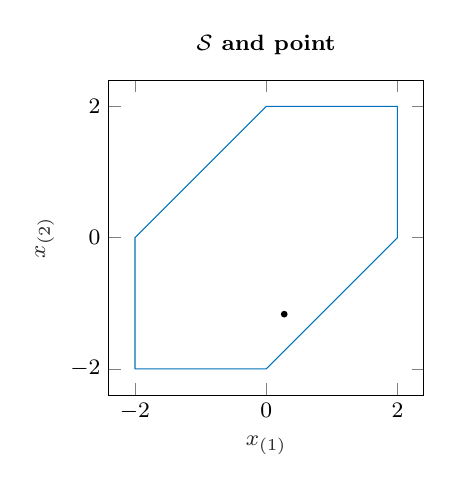
\begin{tikzpicture}
\footnotesize

\begin{axis}[%
width=4cm,
height=4cm,
at={(0in,0in)},
scale only axis,
xmin=-2.4,
xmax=2.4,
xlabel style={font=\color{white!15!black}},
xlabel={$x_{(1)}$},
ymin=-2.4,
ymax=2.4,
ylabel style={font=\color{white!15!black}},
ylabel={$x_{(2)}$},
axis background/.style={fill=white},
title style={font=\bfseries},
title={$\mathcal{S}$ and point}
]
\addplot [color=mycolor1, forget plot]
  table[row sep=crcr]{%
-2	-2\\
0	-2\\
2	0\\
2	2\\
0	2\\
-2	0\\
-2	-2\\
};
\addplot[only marks, mark=*, mark options={}, mark size=1.0000pt, draw=black, forget plot] table[row sep=crcr]{%
x	y\\
0.2747	-1.1657\\
};
\end{axis}
\end{tikzpicture}%
\end{minipage}
\begin{minipage}[t]{0.2\textwidth}
	\vspace{10pt}

	\begin{verbatim}
	Command Window:
		
	p =

    0.2747
   -1.1657
	\end{verbatim}
\end{minipage}
\begin{minipage}[t]{0.3\textwidth}
	\vspace{0pt}
	\centering
	\includetikz{./figures/tikz/set-operations-aux/example_randPoint}
\end{minipage}
\end{center}

\vspace{1cm}

\subsubsubsection{reduce}

The method \operator{reduce} encloses a set by another set with a smaller representation size. Given a set $\mathcal{S} \subset \Rn$, the method \operator{reduce} computes
\begin{equation}
	\operator{reduce}(\mathcal{S},\texttt{method},\texttt{order}) = \overline{\mathcal{S}}, ~~~ \mathcal{S} \subseteq \overline{\mathcal{S}},
	\label{eq:reduce}
\end{equation}
where the representation size of $\overline{\mathcal{S}}$ is smaller than the one of $\mathcal{S}$. The parameter \texttt{method} in \eqref{eq:reduce} is a string that specifies the algorithm to be applied, see \cref{tab:zono_reduction}. The parameter \texttt{order} in \eqref{eq:reduce} is a measure for the desired representation size of the resulting set $\overline{\mathcal{S}}$. Currently, the method \operator{reduce} is implemented for the zonotopic set representations \texttt{zonotope} (see \cref{sec:zonotope}), \texttt{conZonotope} (see \cref{sec:conZonotope}), \texttt{polyZonotope} (see \cref{sec:polynomialZonotopes}), and \texttt{probZonotope} (see \cref{sec:probabilisticZonotopes}), where $\texttt{order} = \frac{p}{n}$ is defined as the division of the number of generator vectors $p$ by the system dimension $n$. Let us demonstrate the method \operator{reduce} by an example:

\begin{center}
\begin{minipage}[t]{0.35\textwidth}
	\vspace{10pt}
	\footnotesize
	\definecolor{mycolor1}{rgb}{0.00000,0.44700,0.74100}%
\definecolor{mycolor2}{rgb}{0.46600,0.67400,0.18800}%
%
\begin{tikzpicture}
\footnotesize
\pgfplotsset{
plotstyle1/.style={color=mycolor1, forget plot},
plotstyle2/.style={color=mycolor2, forget plot}
}
\def\rows{1}
\def\cols{2}
\def\horzsep{1cm}
\def\basepath{./figures/tikz/set-operations-aux/}

\begin{groupplot}[%
group style={rows = \rows, columns = \cols, horizontal sep = \horzsep},
scale only axis,
width=1/\cols*\textwidth -\horzsep,
legend style={legend columns=2,legend to name=legendname, legend cell align=left,/tikz/every even column/.append style={column sep=0.5cm}}
]
\nextgroupplot[xmin=-3,xmax=3,ymin=-3,ymax=3,xlabel={$x_{(1)}$},ylabel={$x_{(2)}$},title={$\mathcal{S}$}]
\input{\basepath example_reduce_11.tikz}
\coordinate (top) at (rel axis cs:0,1);
\nextgroupplot[xmin=-3,xmax=3,ymin=-3,ymax=3,xlabel={$x_{(1)}$},title={$\overline{\mathcal{S}}$}]
\input{\basepath example_reduce_legends.tikz}
\input{\basepath example_reduce_12.tikz}
\coordinate (bot) at (rel axis cs:1,0);
\end{groupplot}
\path (top|-current bounding box.south)--coordinate(legendpos)(bot|-current bounding box.south);
\node at([yshift=-6ex]legendpos) {\pgfplotslegendfromname{legendname}};

\end{tikzpicture}%
\end{minipage}
\begin{minipage}[t]{0.6\textwidth}
	\vspace{0pt}
	\centering
	\includetikz{./figures/tikz/set-operations-aux/example_reduce}
\end{minipage}
\end{center}


\begin{table}[h]
	\caption{Reduction techniques for zonotopic set representations.}
	\centering
	\label{tab:zono_reduction}
	\begin{tabular}{lll}
		\toprule
		\textbf{Technique} & \textbf{Primary use} & \textbf{Reference} \\
		\midrule
		\texttt{cluster} & Reduction to low order by clustering generators & \cite[Sec.~III.B]{Kopetzki2017} \\
		\texttt{combastel} & Reduction of high to medium order & \cite[Sec.~3.2]{Combastel2003} \\
		\texttt{constOpt} & Reduction to low order by optimization & \cite[Sec.~III.D]{Kopetzki2017} \\
		\texttt{girard} & Reduction of high to medium order & \cite[Sec. ~.4]{Girard2005} \\
		\texttt{methA} & Reduction to low order by volume minimization (A) & Meth. A, \cite[Sec.~2.5.5]{Althoff2010a} \\
		\texttt{methB} & Reduction to low order by volume minimization (B) & Meth. B, \cite[Sec.~2.5.5]{Althoff2010a} \\
		\texttt{methC} & Reduction to low order by volume minimization (C) & Meth. C, \cite[Sec.~2.5.5]{Althoff2010a} \\
		\texttt{scott} & Reduction to low order  & \cite[Appendix]{Scott2016} \\
		\texttt{pca} & Reduction of high to medium order using PCA & \cite[Sec.~III.A]{Kopetzki2017} \\
		\bottomrule
	\end{tabular}
\end{table}


\subsubsubsection{supportFunc}

The method \operator{supportFunc} computes the support function for a specific direction. Given a set $\mathcal{S} \in \Rn$ and a vector $l \in \Rn$, the support function is defined as
\begin{equation*}
	\operator{supportFunc}(\mathcal{S},l) = \max_{x \in \mathcal{S}} ~l^T~x.
\end{equation*}
The function also supports the computation of the lower bound, which can be calculated using the flag \texttt{'lower'}:
\begin{equation*}
	\operator{supportFunc}(\mathcal{S},l,\texttt{'lower'}) = \min_{x \in \mathcal{S}} ~l^T~x.
\end{equation*}
Additionally, one can return both the lower and upper bounds by using the flag \texttt{'range'}.
Let us demonstrate the method \operator{supportFunc} by an example:

\begin{center}
\begin{minipage}[t]{0.40\textwidth}
	\vspace{10pt}
	\footnotesize
	% This file was created by matlab2tikz.
%
\definecolor{mycolor1}{rgb}{0.00000,0.44700,0.74100}%
\definecolor{mycolor2}{rgb}{0.85000,0.32500,0.09800}%
%
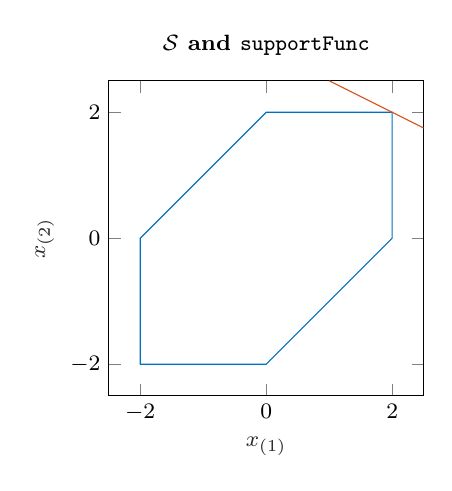
\begin{tikzpicture}
\footnotesize

\begin{axis}[%
width=4cm,
height=4cm,
at={(0in,0in)},
scale only axis,
xmin=-2.5,
xmax=2.5,
xlabel style={font=\color{white!15!black}},
xlabel={$x_{(1)}$},
ymin=-2.5,
ymax=2.5,
ylabel style={font=\color{white!15!black}},
ylabel={$x_{(2)}$},
axis background/.style={fill=white},
title style={font=\bfseries},
title={$\mathcal{S}$ and \texttt{supportFunc}}
]
\addplot [color=mycolor1, forget plot]
  table[row sep=crcr]{%
-2	-2\\
0	-2\\
2	0\\
2	2\\
0	2\\
-2	0\\
-2	-2\\
};
\addplot [color=mycolor2, forget plot]
  table[row sep=crcr]{%
2.5	1.75\\
1	2.5\\
};
\end{axis}
\end{tikzpicture}%
\end{minipage}
\begin{minipage}[t]{0.2\textwidth}
	\vspace{10pt}

	\begin{verbatim}
	Command Window:
		
	res = 6
	\end{verbatim}
\end{minipage}
\begin{minipage}[t]{0.3\textwidth}
	\vspace{0pt}
	\centering
	\includetikz{./figures/tikz/set-operations-aux/example_supportFunc}
\end{minipage}
\end{center}


\subsubsubsection{plot}

The method \operator{plot} visualizes a 2-dimensional projection of the boundary of a set. Given a set $\mathcal{S} \subset \Rn$, the method \operator{plot} supports the following syntax:
\begin{equation*}
	\begin{split}
		&\texttt{han} = \operator{plot}(\mathcal{S}), \\
		&\texttt{han} = \operator{plot}(\mathcal{S},\texttt{dims}), \\
		&\texttt{han} = \operator{plot}(\mathcal{S},\texttt{dims},\texttt{linespec}), \\
		&\texttt{han} = \operator{plot}(\mathcal{S},\texttt{dims},\texttt{namevaluepairs}), \\
	\end{split}
\end{equation*}
where \texttt{han} is a handle to the plotted MATLAB graphics object and the additional input arguments are defined as

\begin{itemize}
	\item \texttt{dims}: Integer vector $\texttt{dims} \in \mathbb{N}_{\leq n}^2$ specifying the dimensions for which the projection is visualized (default value: \texttt{dim = [1 2]}).
	\item \texttt{linespec}: (optional) line specifications, e.g., \texttt{'--*r'}, as supported by MATLAB\footnote{\url{https://de.mathworks.com/help/matlab/ref/linespec.html}}.
	\item \texttt{namevaluepairs}: (optional) further specifications as name-value pairs, e.g.,
	\texttt{'LineWidth',2} and \texttt{'FaceColor',[.5 .5 .5]}, as supported by MATLAB.
	If the plot is not filled, these are the built-in
	Line Properties\footnote{\url{https://de.mathworks.com/help/matlab/ref/matlab.graphics.chart.primitive.line-properties.html}},
	if the plot is filled, they correspond to the Patch Properties\footnote{\url{https://de.mathworks.com/help/matlab/ref/matlab.graphics.primitive.patch-properties.html}}.
\end{itemize}

Let us demonstrate the method  \operator{plot} by an example:

\begin{center}
\begin{minipage}[t]{0.40\textwidth}
	\vspace{10pt}
	\footnotesize
	% This file was automatically created from the m-file 
% "m2tex.m" written by USL. 
% The fontencoding in this file is UTF-8. 
%  
% You will need to include the following two packages in 
% your LaTeX-Main-File. 
%  
% \usepackage{color} 
% \usepackage{fancyvrb} 
%  
% It is advised to use the following option for Inputenc 
% \usepackage[utf8]{inputenc} 
%  
  
% definition of matlab colors: 
\definecolor{mblue}{rgb}{0,0,1} 
\definecolor{mgreen}{rgb}{0.13333,0.5451,0.13333} 
\definecolor{mred}{rgb}{0.62745,0.12549,0.94118} 
\definecolor{mgrey}{rgb}{0.5,0.5,0.5} 
\definecolor{mdarkgrey}{rgb}{0.25,0.25,0.25} 
  
\DefineShortVerb[fontfamily=courier,fontseries=m]{\$} 
\DefineShortVerb[fontfamily=courier,fontseries=b]{\#} 
  
\noindent       
 $$\color{mgreen}$% set S$\color{black}$$\\
 $S = zonotope([0 1 1 0;$\color{mblue}$ ...$\color{black}$$\\
 $              0 1 2 1;$\color{mblue}$ ...$\color{black}$$\\
 $              0 1 0 1]);$\\
 $          $\\
 $$\color{mgreen}$% visualization$\color{black}$$\\
 $plot(S,[1,3],$\color{mred}$'--r'$\color{black}$);$\\
  
\UndefineShortVerb{\$} 
\UndefineShortVerb{\#}
\end{minipage}
\begin{minipage}[t]{0.3\textwidth}
	\vspace{0pt}
	\centering
	\includetikz{./figures/tikz/set-operations-aux/example_plot}
\end{minipage}
\end{center}


\vspace{1cm}

\subsubsubsection{project}

The method \operator{project} projects a set to a lower-dimensional, axis-aligned subspace. Given a set $\mathcal{S} \subset \Rn$ and a vector of subspace indices $\texttt{dims} \in \mathbb{N}_{\leq n}^m$, the method \operator{project} returns
\begin{equation*}
	\operator{project}(\mathcal{S},\texttt{dims}) = \Big \{ [s_{(\texttt{dims}_{(1)})},\dots,s_{(\texttt{dims}_{(m)})}]^T ~\Big |~ s \in \mathcal{S} \Big \} \subset \R^m,
\end{equation*}
where $s_{(i)}$ denotes the i-th entry of vector $s$. Let us demonstrate the method  \operator{project} by an example:

\begin{center}
\begin{minipage}[t]{0.40\textwidth}
	\vspace{10pt}
	\footnotesize
	% This file was automatically created from the m-file 
% "m2tex.m" written by USL. 
% The fontencoding in this file is UTF-8. 
%  
% You will need to include the following two packages in 
% your LaTeX-Main-File. 
%  
% \usepackage{color} 
% \usepackage{fancyvrb} 
%  
% It is advised to use the following option for Inputenc 
% \usepackage[utf8]{inputenc} 
%  
  
% definition of matlab colors: 
\definecolor{mblue}{rgb}{0,0,1} 
\definecolor{mgreen}{rgb}{0.13333,0.5451,0.13333} 
\definecolor{mred}{rgb}{0.62745,0.12549,0.94118} 
\definecolor{mgrey}{rgb}{0.5,0.5,0.5} 
\definecolor{mdarkgrey}{rgb}{0.25,0.25,0.25} 
  
\DefineShortVerb[fontfamily=courier,fontseries=m]{\$} 
\DefineShortVerb[fontfamily=courier,fontseries=b]{\#} 
  
\noindent      
 $$\color{mgreen}$% set S$\color{black}$$\\
 $S = interval([1;2;5;0],$\color{mblue}$ ...$\color{black}$$\\
 $             [3;3;7;2]);$\\
 $          $\\
 $$\color{mgreen}$% projection$\color{black}$$\\
 $res = project(S,[1 3 4]);$\\ 
  
\UndefineShortVerb{\$} 
\UndefineShortVerb{\#}
\end{minipage}
\begin{minipage}[t]{0.25\textwidth}
	\vspace{10pt}

	\begin{verbatim}	
	Command Window:
	
	res = 
 [1.00000,3.00000]
 [5.00000,7.00000]
 [0.00000,2.00000]
	\end{verbatim}
\end{minipage}
\end{center}

A set can be projected into a higher-dimensional space using the function \operator{projectHighDim},
where the new dimensions are bounded at 0.
On the other hand, the function \operator{lift} lifts the set into a higher-dimensional space with unbounded new dimensions.